\chapter{Introduction}

\section{Motivation}
Revealing the structure of hierarchical organized data is a complex task where many approaches already exists. It is still an active research area as data scientists are facing ever greater challenges when analyzing large hierarchical datasets. One example is the Human Disease Network \cite{zhou_human_2014} which is a hierarchical network of disorders and disease genes with approximately 3000 nodes on two different hierarchy layers. Figure \ref{fig:Human_Disease_Network} shows us the representation of the data in a common two-dimensional layout. In this representation, the classes of disorders are coded by color. 
Another dataset with a similar structure can be seen in Figure \ref{fig:original2DdiseaseNet}, here the clusters of different diseases are grouped by boxes.\\ 
Depiction of hierarchical network structure in 2D faces us with many challenges. The biggest one is visual clutter also called hairball effect which reduces the legibility of the network information, therefore it is difficult to determine node-node relationships and hierarchic-associations as well as hierarchic relationships which are crucial in analyzing hierarchical network data. In Figure \ref{fig:Human_Disease_Network} we can see this effect on the green nodes. The graph in Figure \ref{fig:original2DdiseaseNet} solves this problem by hiding links between child nodes from different boxes which is also not optimal.

\begin{figure}[h]
    \centering
    \begin{subfigure}[b]{0.4\columnwidth}
        \centering
        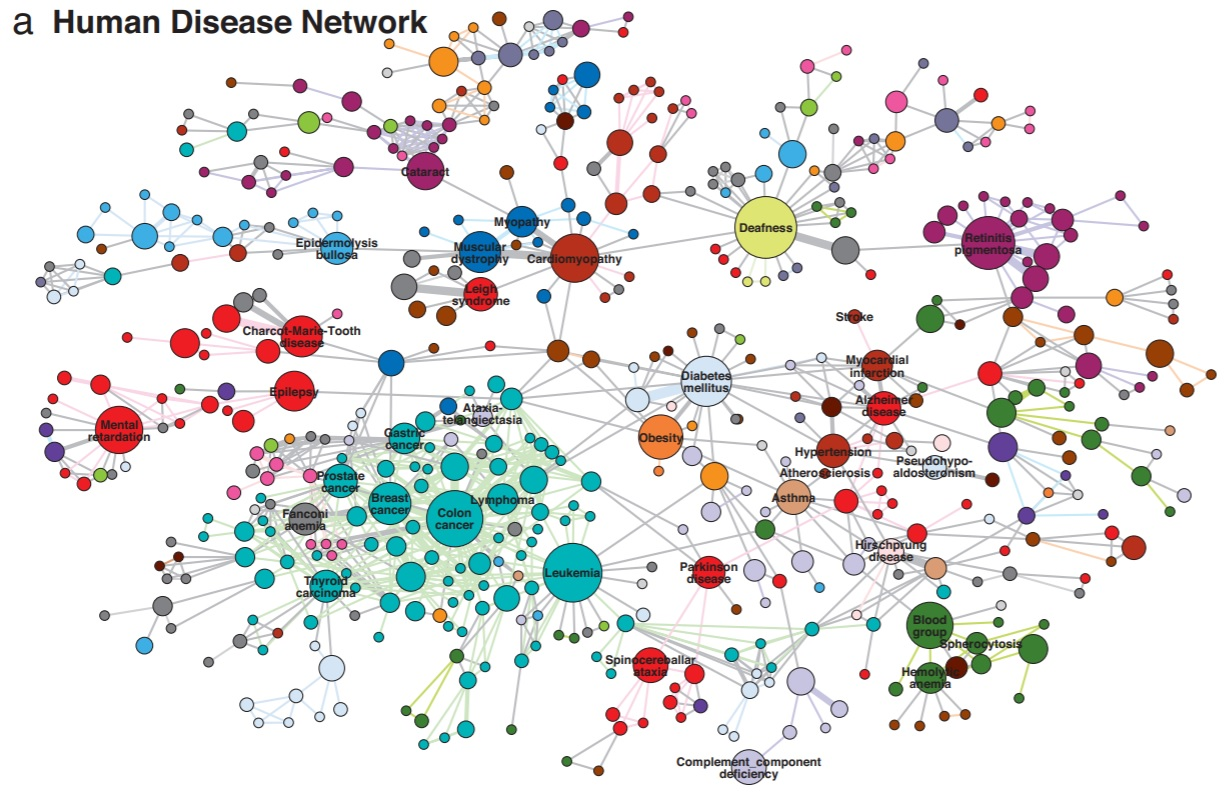
\includegraphics[width=\textwidth, trim={0 0 9cm 0},clip]{graphics/Human_Disease_Network.jpg}
        \subcaption{Human Disease Network \cite{zhou_human_2014}}
        \label{fig:Human_Disease_Network}
    \end{subfigure}
    \begin{subfigure}[b]{0.5\columnwidth}
      \centering
      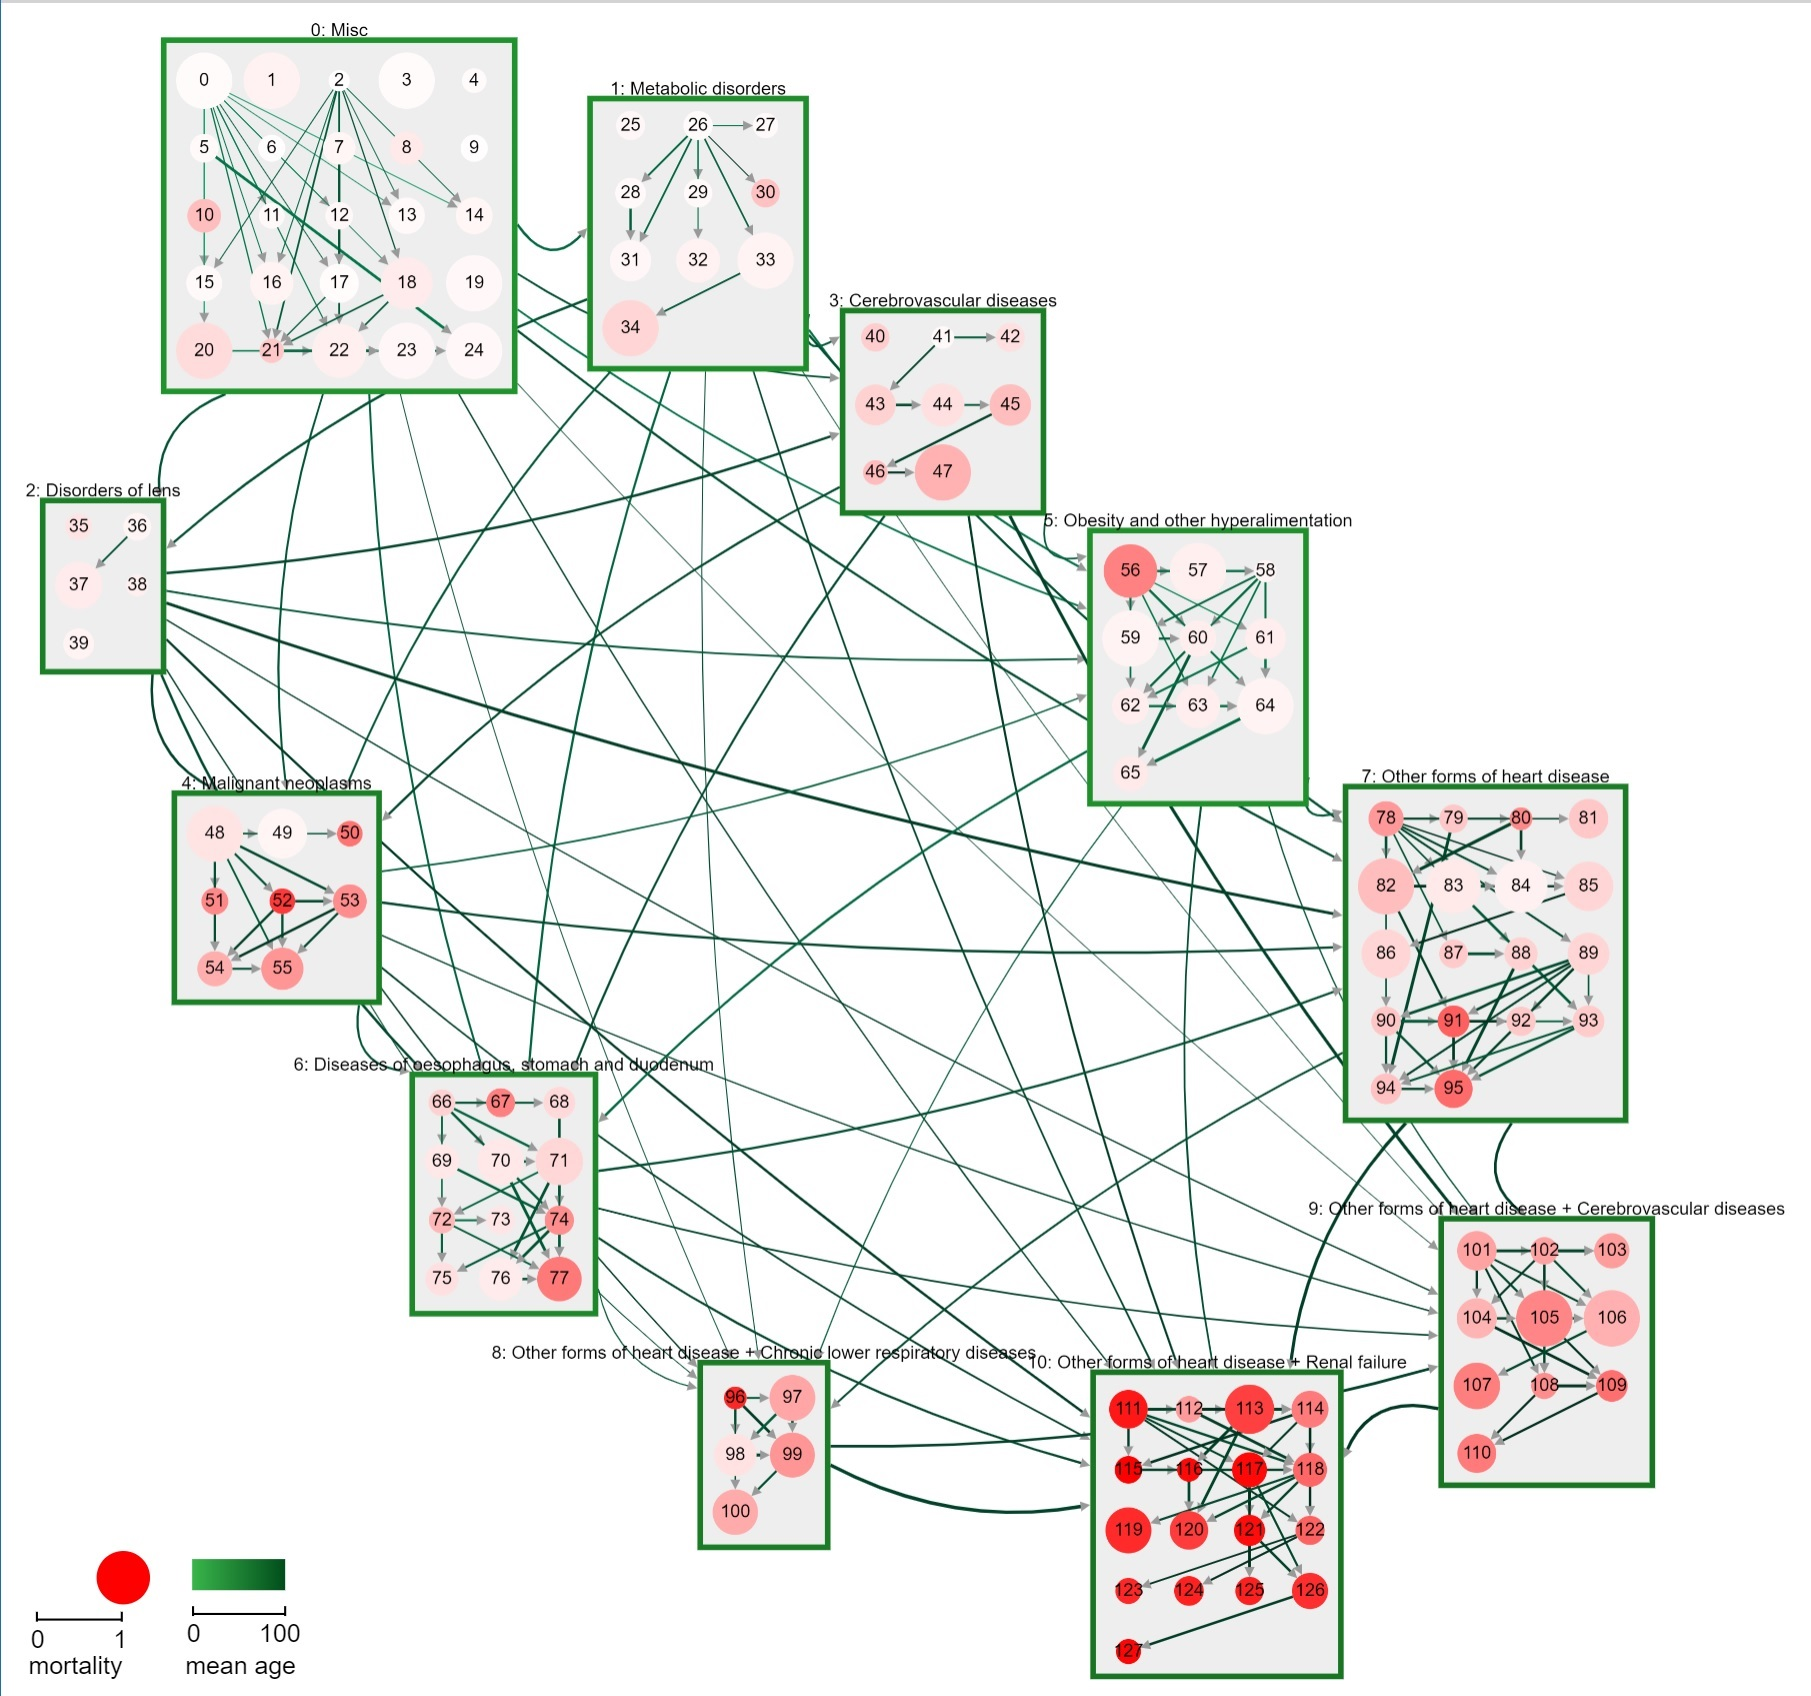
\includegraphics[width=\textwidth]{graphics/original2DdiseaseNet.jpg}
      \subcaption{a comorbidity network of diagnoses related to diabetes melitus}
      \label{fig:original2DdiseaseNet}
    \end{subfigure}
    \caption[Optional caption for the figure list (often used to abbreviate long captions)]{Example visualizations of hierarchical network datasets in two dimensions. Both consists of two hierarchical layers.} % Remove the [...] argument if the original caption should be used in the figure list.
    \label{fig:intro} 
  \end{figure}

3D information visualization allows us to expand the user experience of traditional 2D graphs. As Brath describes in his paper \cite{brath_3d_2014} there are many advantages and opportunities when using three-dimensional visualizations.
By using an additional axis the visualization has more space to distribute all the data and reduce clutter in the first place before applying specialized layouts. The mental model of the data gets improved which leads to a better cluster detection, conformation and general overview of the data. 
Some visualization also use the additional axis to encode an extra attribute by its position, this can be seen in the “3D space time cube” \cite{brath_3d_2014} here the temporal information is encoded on the Z axis another common usage is a 3D scatter plot.
In three-dimensional layouts, the perspective of the visualization has to be reconsidered. Usually the user looks from the outside with a bird's eye view at the visualization. In 3D however the viewer can be placed right inside our graph, this enables us to utilize new navigation and interaction possibilities.

Still, all these opportunities also involve new challenges: navigation inside a hierarchically structured 3D scene, occlusion of elements in an 3D perspective view, selection of objects for displaying details and the lack of a reference point in an abstract three-dimensional space. Brath \cite{brath_3d_2014} already stated that immersive interfaces could help to overcome these issues.\label{chap:advantages_VR}
We believe that the recent developments in virtual reality hardware and frameworks offer great potential to address these challenges. 
We can see the benefits of VR based visualizations in various publications. Bowman et al. \cite{bowman_virtual_2007} examined the impact of VR techniques, like stereoscopic images, interaction with the virtual world and head movement, can have on users. 
Recently Kraus et al. \cite{kraus_impact_2020} did a study on the effect of immersion for detecting clusters in a scatter plot. Their results show that VR based visualization systems have real world advantages in terms of time needed to get an overview of the data compared to traditional 2D- and 3D information visualization. 
 
\section{Aim of the Work}

Our goal is to implement a visualization for hierarchical network data that allows users take the benefits of 3D information visualization and opportunities of virtual reality technology to dive right into the data. We believe the combination of both concepts complete each other well because VR based technology can be used to solve the subsequent challenges from 3D information visualization and therefore enable data scientists to optimize their data analysis tasks. 
Our aim was to design a customized graph layout that calculates the position and size of each node by the hierarchical structure: child nodes are nested within its parent node. 
In addition, visual clutter by overlapping of nodes and links should be prevented. 
Furthermore, the exploration of the resulting graph should be possible with room scaled virtual reality devices like the HTC Vive, requiring optimized navigation, filtering and brushing methods to enhance the graph exploration user experience.

\section{Methodology}
In order to achieve the proclaimed goal we defined our own 3D layout. The result can be seen in Figure \ref{fig:conceptSketch}. Our core concepts are the following: 
\begin{itemize}
    \item We render each hierarchy layer as a three-dimensional structure instead a flat surface as seen in many multilayer network visualizations for example Figure \ref{fig:2dmultilayerVis}. This enables us to use the entire volume to evenly distribute our nodes and links of the network and also enabling the representation of cluster formations within a hierarchy layer. Furthermore, it helps us to reduce cluttering of nodes and links.
    \item For the hierarchical relationship, we use the concept of nesting child nodes into parent nodes as seen in tree map visualizations for example Figure \ref{fig:hierarchicalCirclePlot}. However, we use 3D spheres instead of 2D circles. 
    \item In addition, our visualization is not limited to two hierarchical layers as seen in the Figure, but rather is able to display $n$ hierarchical layers. To achieve this we simply repeat the process of nesting child nodes into parents for each layer.
    \item To dynamically build this layout for any given data as input we developed a custom force based system. It consists of various attracting forces for nodes of the same hierarchical layer and parent, as well as repelling forces between nodes of different parents in the same hierarchical layer.
\end{itemize}
%repelling and attracting
As the context of 3D layout introduces new challenges for navigation and interaction we had to come up with some ideas to solve this: 
\begin{itemize}
    \item The main target of our visualization system is a room scaled virtual reality experience.
    \item For user input we fully utilize the tracking capabilities of the HTC Vive controllers. Selection of nodes and links is possible with a virtual “laser pointer” attached to the user's controller in the scene.
    \item For navigation, we provide two kinds of navigation methods: One for bridging larger distances like flying to a specific node selected by the user or flying to the hierarchical parent node. Additional, a free flying navigation that allows the user to fine tune their position.
    \item Links between nodes are possible in one network but also to other networks of the same hierarchical layer. The visibility of the links is changed automatically by the position of the user and manually by selecting a node with the virtual laser pointer during the exploration process. 
\end{itemize}
Our concept of nested hierarchical layers implies that nodes and links of inner layers get smaller for each iteration of nesting. This introduces a new problem as after a few iterations the nodes and links in the virtual scene are too small to recognize. In a 2D layout this is usually solved with zooming. However, as this is not possible within a 3D layout we came up with two additional concepts: 
\begin{itemize}
    \item The free flying navigation speed is adaptive. On entering an inner hierarchical layer the speed is reduced and on leaving increased.
    \item In VR, navigation also always happens through movement in the real world, e.g. walking around. We can dynamically adjust the flying speed, but obviously we can not adjust the physical movement speed of the user in the real world. Furthermore, the size of objects in a virtual scene is always directly linked to real world sizes. (e.g. 1 virtual unit is 1 meter in the real world). To solve this problem we also dynamically adjust the size of the entire scene while exploring the graph. Increasing the scale on entering an inner layer and reducing on leaving. 
\end{itemize}

%As stated by Sadana et al. \cite{sadana_redefining_2016}, it is also important to explore how existing techniques can be applied to new platforms like virtual reality devices. To this end, we take existing already well established 2D visualization techniques combine them and extend the result into the three-dimensional space. We adapted a tree map visualization (see Figure \ref{fig:hierarchicalCirclePlot}) for visualizing the hierarchical aspect and a flat multilayer network (see Figure \ref{fig:2dmultilayerVis}) for the network relationships.  

\begin{figure}[h]
    \centering
    \begin{subfigure}[b]{0.40\columnwidth}
        \centering
        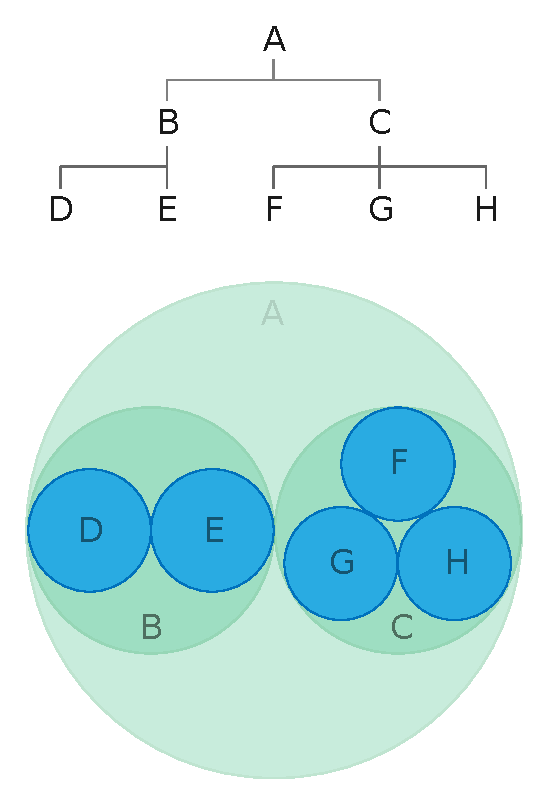
\includegraphics[width=\textwidth, trim={0 0 0 4.3cm},clip]{graphics/circle_packing.pdf}
        \subcaption{Hierarchical circle packing plot \cite{ribecca_circle_nodate}}
        \label{fig:hierarchicalCirclePlot}
    \end{subfigure}
    \begin{subfigure}[b]{0.50\columnwidth}
      \centering
      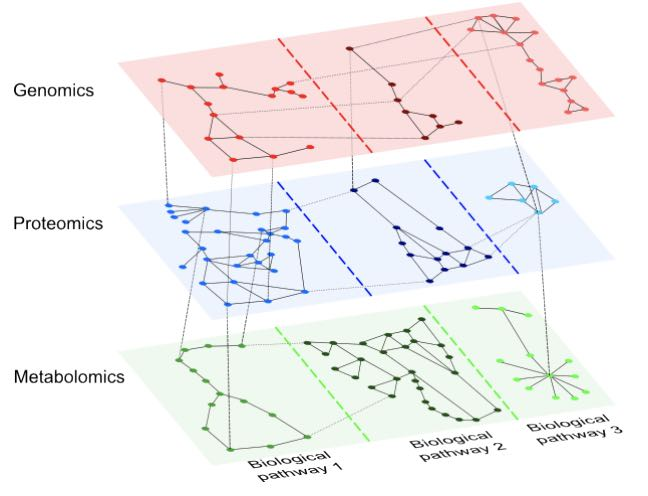
\includegraphics[width=\textwidth]{graphics/2dmultilayerVis.jpg}
      \subcaption{multilayer network visualization \cite{ghoniem_state_2019}}
      \label{fig:2dmultilayerVis}
    \end{subfigure}
    \caption[Optional caption for the figure list (often used to abbreviate long captions)]{(a) shows a possible visualization for hierarchical structures, (b) shows a visualization for networks with multiple layers} % Remove the [...] argument if the original caption should be used in the figure list.
    \label{fig:referenceVisualizations} 
  \end{figure}

\begin{figure}[h]
    \centering
    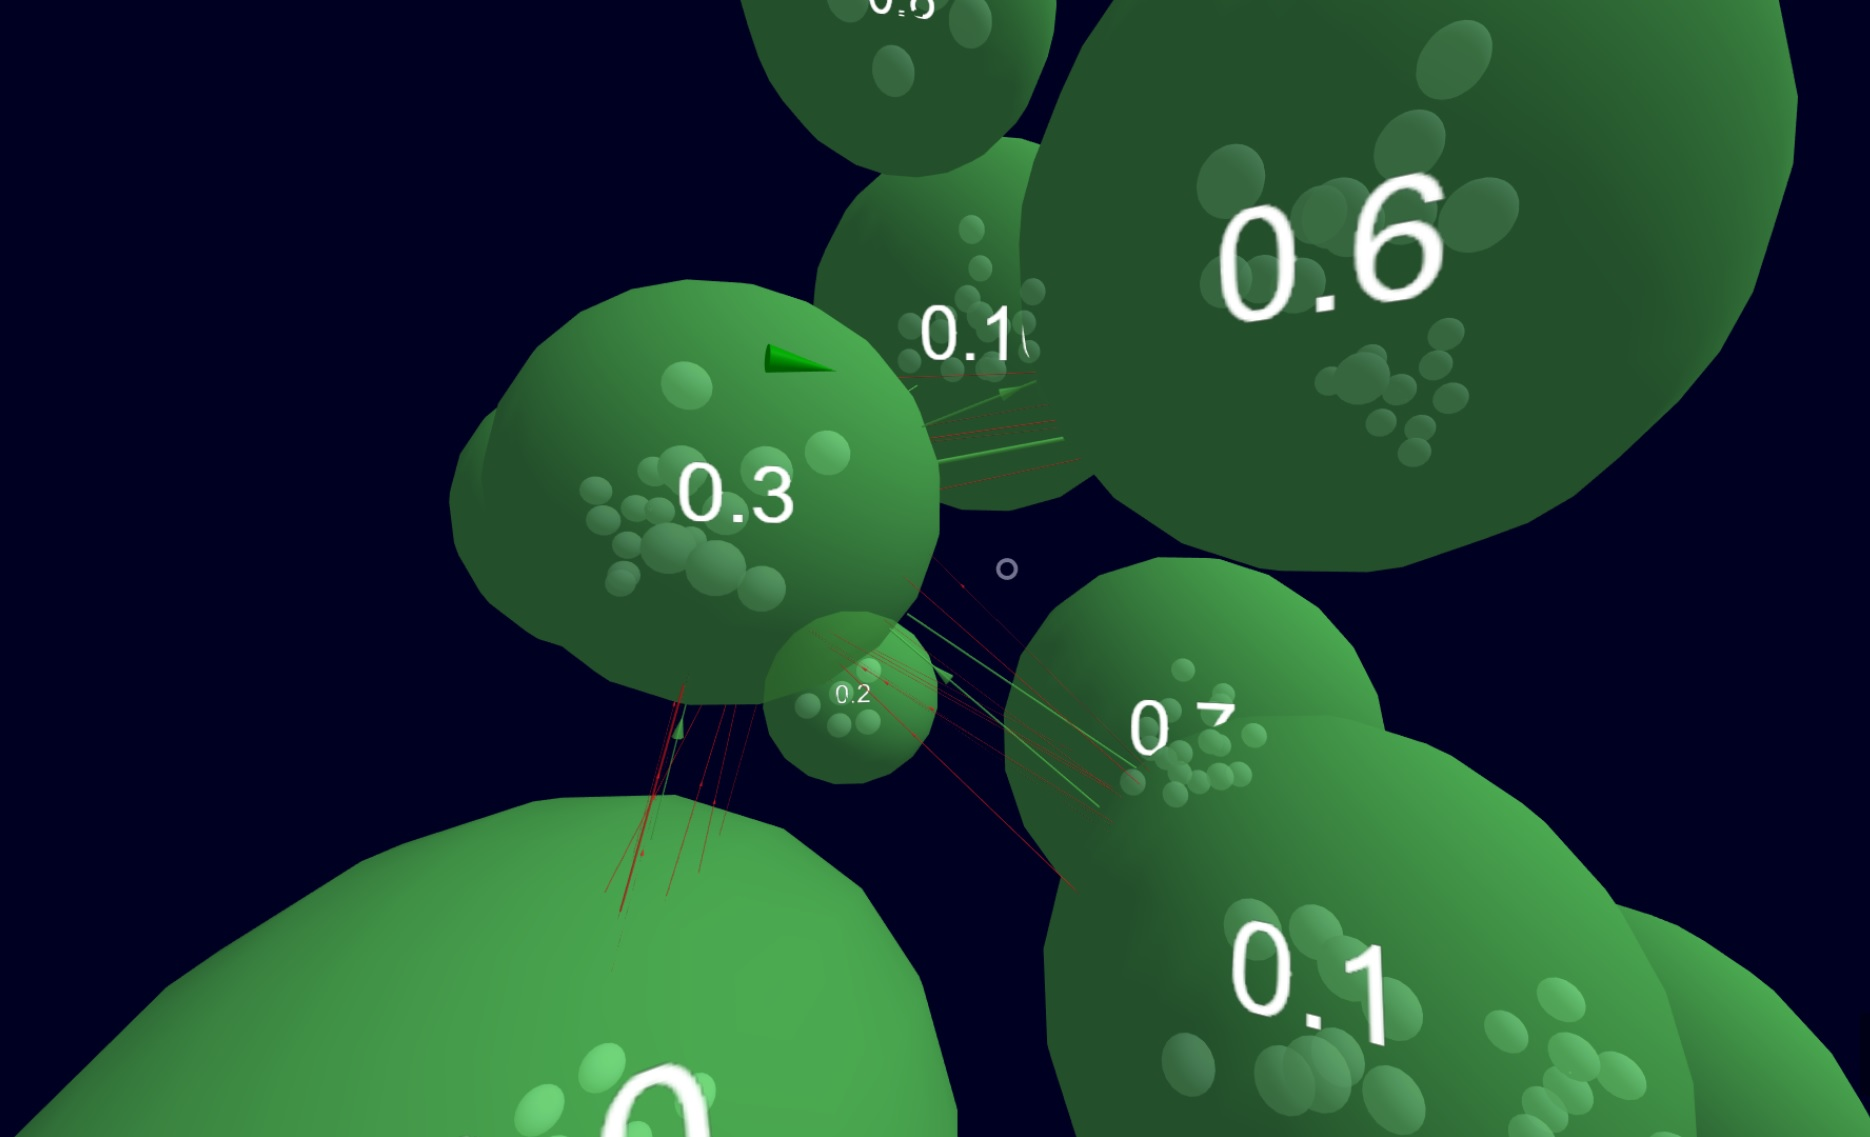
\includegraphics[width=1\textwidth]{graphics/conceptScreenshot.jpg}
    \caption{Screenshot of the comorbidity network dataset from \ref{fig:original2DdiseaseNet} in our hierarchical network visualization. On the screenshot only edges from node 0.3 are displayed.} % Remove the [...] argument if the original caption should be used in the figure list.
    \label{fig:conceptSketch} 
\end{figure}

To evaluate our results we gathered feedback from multiple people including ourselves on overview of the visualization, navigation, interaction and motion sickness. However, a full user study is out of scope of this thesis.